\setcounter{section}{31}
\section{Конденсация ориентированного графа, ацикличность}
\textbf{Определение} \textit{Кондексацией} ориентированного графа называется граф, построенный таким образом:
\begin{itemize}
    \item [1] Выделяем компоненты сильной связности графа
    \item[2] Сжимаем компоненты сильной связности до вершин
    \item[3] Оставляем ребра между разными КСС, убираем кратные ребра
\end{itemize}
\textbf{Утверждение}\\
Конденсированный граф ацикличен. 
\\
$\blacktriangle \ $Предположим, это не так, тогда существует цикл между разными КСС
\begin{center}
    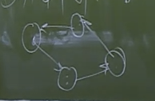
\includegraphics[width=5cm,height=4cm]{images/32_alg13.PNG}
    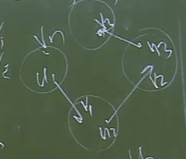
\includegraphics[width=5cm,height=4cm]{images/32_alg14.PNG}
\end{center}
Пусть это цикл 
\\
$u_1 \rightarrow v_1$ \\ $u_2 \rightarrow v_2$ \\ ... \\ $u_n \rightarrow v_n$, \\Тогда, так как эти ребра соединяют компоненты сильной связности, из первой компоненты цикла можно добраться до любой компоненты оставшейся части цикла, а значит, и любой вершины из компонент сильной связности, входящих в цикл. Аналогично для второй, третьей и т.д. компоненты из цикла. То есть компоненты, образующие цикл, являются КСС, а значит, разбиение на КСС было некорректным. Противоречие $\ \blacksquare$